\documentclass[11pt,a4paper]{article}

% --- encoding & fonts ---
\usepackage[utf8]{inputenc}
\usepackage[T1]{fontenc}
\usepackage{lmodern}

% --- layout ---
\usepackage[margin=2.5cm]{geometry}
\usepackage{microtype}

% --- math ---
\usepackage{amsmath,amssymb}

% --- figures & tables ---
\usepackage{graphicx}
\usepackage{float}
\usepackage{booktabs}
\usepackage{tabularx}
\usepackage{caption}
\usepackage{subcaption}
\usepackage{xcolor}
\usepackage{rotating}
\usepackage{multirow}

% --- code listings ---
\usepackage{listings}
\lstset{
  basicstyle=\ttfamily\small,
  breaklines=true,
  frame=single,
  columns=fullflexible,
  showstringspaces=false,
  literate={->}{{\ensuremath{\to}}}2
}

% --- references ---
\usepackage{hyperref}
\usepackage{cleveref}

% ── Part II entity macros ───────────────────────────────────────────────────
% Object types
\newcommand{\otBranches}{\texttt{branches}}
\newcommand{\otUsers}{\texttt{users}}
\newcommand{\otFiles}{\texttt{files}}
\newcommand{\otFileVersions}{\texttt{file versions}}

% Event types
\newcommand{\etCommit}{\texttt{commit}}
\newcommand{\etPull}{\texttt{pull}}
\newcommand{\etMerge}{\texttt{merge}}
\newcommand{\etPush}{\texttt{push}}

% Constraints
\newcommand{\Cone}{C1}
\newcommand{\Ctwo}{C2}
\newcommand{\Cthree}{C3}

% OCPN names
\newcommand{\None}{$N_1$}
\newcommand{\Ntwo}{$N_2$}

% User name
\newcommand{\userCameron}{\textit{Cameron}}

% Log names
\newcommand{\logL}{$L$}
\newcommand{\logLone}{$L_1$}
\newcommand{\logLuone}{$L_1^{\text{Cameron}}$}
\newcommand{\logLtwo}{$L_2$}

% Placeholder box for missing figures / tables
\newcommand{\placeholder}[2][8cm]{%
  \fbox{\parbox{#1}{\centering\vspace{1.5cm}\textcolor{red}{\textbf{TODO:} #2}\vspace{1.5cm}}}%
}

% Inline TODO marker
\newcommand{\TODO}[1]{\textcolor{red}{\textbf{[TODO: #1]}}}

% ── GSLPN firing-sequence trace table (Q3) ──────────────────────────────────
% Usage:
%   \begin{pathtrace}{Path $\pi_1$: caption text}{tab:label}
%     0 & $\langle\rangle$   & $M_0=\{p_1\}$      & --      & --                       \\
%     1 & $\langle a\rangle$ & $M_1=\{p_2\}$      & $t_a$   & $1$                      \\
%     2 & $\langle a,d\rangle$ & $M_2=\{p_3,p_4\}$ & $t_d$ & $\frac{w_d}{w_d+w_x}$      \\
%   \end{pathtrace}
% Columns: Step | Trace so far | Marking | Transition fired | Probability
\newenvironment{pathtrace}[2]{%
  \def\pathtracecaption{#1}%
  \def\pathtracelabel{#2}%
  \begin{table}[H]
  \centering
  \begin{tabular}{@{}clccc@{}}
    \toprule
    Step & Trace so far & Marking & Transition fired & $P(\text{step})$ \\
    \midrule
}{%
    \bottomrule
  \end{tabular}
  \caption{\pathtracecaption}
  \label{\pathtracelabel}
  \end{table}
}

\title{Advanced Process Mining --- Assignment Part II}
\author{Group $\langle$GroupID$\rangle$ \\ $\langle$Member 1$\rangle$, $\langle$Member 2$\rangle$, $\langle$Member 3$\rangle$}
\date{\today}

\begin{document}
\maketitle
\tableofcontents
\newpage

% ─────────────────────────────────────────────────────────────────────────────
% Question 1: Declare  (NOT our responsibility — placeholder only)
% ─────────────────────────────────────────────────────────────────────────────
% \section{Question 1: Declare}

% ─────────────────────────────────────────────────────────────────────────────
% Question 2: EMSC  (NOT our responsibility — placeholder only)
% ─────────────────────────────────────────────────────────────────────────────
% \section{Question 2: EMSC}

% ─────────────────────────────────────────────────────────────────────────────
\section{Question 3: Trace Probabilities in GSLPNs}
% Q3: Trace Probabilities in GSLPNs
% Solved by q3_gslpn.py: the net below is entered by hand from the figure on
% p.6 of the assignment PDF, then a generic marking-graph / embedded-DTMC
% solver computes (a) and (b).
%
% Trace: sigma = <a, d, c, e, f>

\begin{figure}[H]
      \centering
      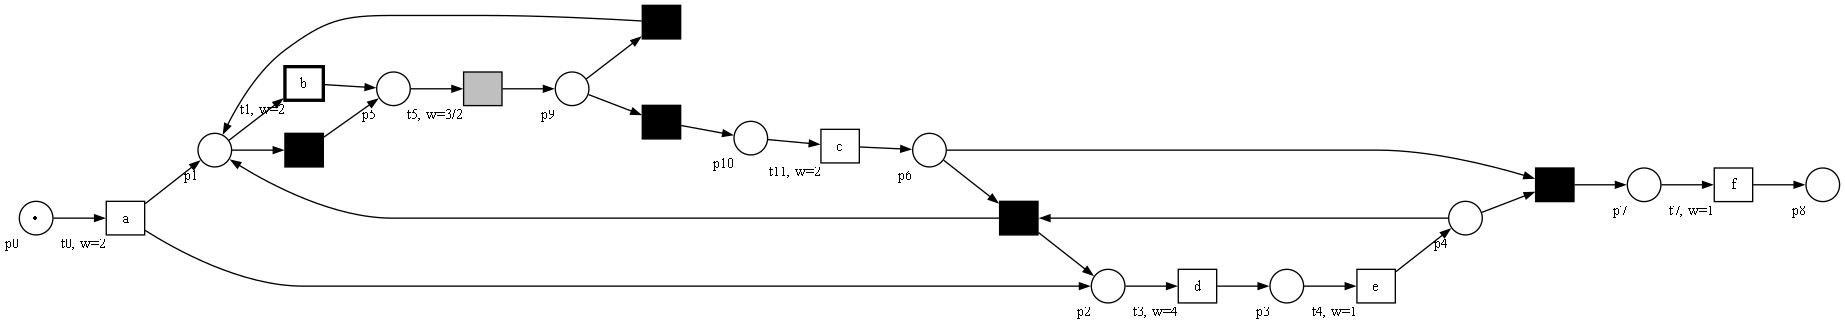
\includegraphics[width=\textwidth,height=0.4\textheight,keepaspectratio]{figures/gslpn_net.png}
      \caption{The GSLPN from the assignment (p.6), redrawn from the encoding used by
            \texttt{q3\_gslpn.py}. Layout differs from the
            original figure (auto-generated left-to-right), but the places, transitions,
            weights and arcs are identical. Legend: plain box = timed, thick-bordered
            box = immediate (visible), grey box = $\tau$ and timed, black box = $\tau$
            and immediate.}
      \label{fig:gslpn}
\end{figure}

\subsection*{(a) Stochastic path with highest probability}
\label{sec:q3a}

Computed by \texttt{q3\_gslpn.py}: every enabled transition set is
split into immediate/timed per the priority rule, the winning class races by weight, and the
highest-probability firing sequence projecting onto $\sigma$ is found with a Dijkstra variant
that maximizes a product of probabilities instead of minimizing a sum of costs.

\begin{pathtrace}{Path $\pi_1$: $\langle a,d,c,e,f\rangle$ via $(t_0,t_2,t_3,t_5,t_{10},t_{11},t_4,t_6,t_7)$}{tab:q3a-pi1}
      0 & $\langle\rangle$           & $M_0 = \{p_0\}$        & --      & --             \\
      1 & $\langle a\rangle$         & $M_1 = \{p_1,p_2\}$    & $t_0$   & $1$            \\
      2 & $\langle a\rangle$         & $M_2 = \{p_2,p_5\}$    & $t_2$   & $\frac{3}{5}$  \\
      3 & $\langle a,d\rangle$       & $M_3 = \{p_3,p_5\}$    & $t_3$   & $\frac{8}{11}$ \\
      4 & $\langle a,d\rangle$       & $M_4 = \{p_3,p_9\}$    & $t_5$   & $\frac{3}{5}$  \\
      5 & $\langle a,d\rangle$       & $M_5 = \{p_3,p_{10}\}$ & $t_{10}$ & $\frac{1}{4}$ \\
      6 & $\langle a,d,c\rangle$     & $M_6 = \{p_3,p_6\}$    & $t_{11}$ & $\frac{2}{3}$ \\
      7 & $\langle a,d,c,e\rangle$   & $M_7 = \{p_4,p_6\}$    & $t_4$   & $1$            \\
      8 & $\langle a,d,c,e\rangle$   & $M_8 = \{p_7\}$        & $t_6$   & $\frac{1}{3}$  \\
      9 & $\langle a,d,c,e,f\rangle$ & $M_9 = \{p_8\}$        & $t_7$   & $1$            \\
\end{pathtrace}

\[
      P(\pi_1) = 1\cdot\tfrac{3}{5}\cdot\tfrac{8}{11}\cdot\tfrac{3}{5}\cdot\tfrac{1}{4}\cdot\tfrac{2}{3}\cdot1\cdot\tfrac{1}{3}\cdot1 = \frac{4}{275} \approx 0.0145
\]

Step 2 is a race between $t_1$ ($b$, $w=2$) and $t_2$ ($\tau$, $w=3$); firing $t_1$ would
introduce a $b$ that $\sigma$ does not contain, so only $t_2$ can extend a match, at probability
$\frac{3}{5}$. At every point where $p_9$ has a token (step 4$\to$5), the alternative is the
silent loop $t_9$ ($w=3$) back to $p_1$: since every extra loop multiplies the remaining
probability by a factor strictly less than 1 (and re-visits $p_1$ without ever adding to the
match, since $t_1/b$ still cannot fire), looping can never exceed the direct continuation
through $t_{10}$. The same argument rules out $t_8$ ($w=2$) at step 8: taking it would force a
second, unmatched $d$/$e$/$c$ before any further progress is possible. Hence $\pi_1$ above is
the unique candidate and thus the maximum: $P(\pi_1) = \frac{4}{275} \approx 1.45\%$.



\subsection*{(b) Probability of observing trace $\sigma$}
\label{sec:q3b}

Unlike (a), $\pi_1$ is not the only path projecting onto $\sigma$: the silent loop
$t_9 \to p_1 \to t_2 \to p_5 \to t_5 \to p_9$ can repeat any number of times (always avoiding
$t_1/b$) before finally taking $t_{10}$, and its position can interleave differently with the
$d/e$ branch -- both without changing the visible trace. This is an infinite family of paths, so
$P(\sigma)$ is computed (not enumerated) as the absorption probability, into the accepting
state, of the embedded DTMC restricted to $\sigma$-consistent transitions -- i.e.\ the solution
of the linear system $x_s = \sum_{\text{edges } s\to s'} p\cdot x_{s'}$ over the (finite, 17-state)
reachable marking graph, with $x_{\text{accept}}=1$:
\[
      P(\sigma) = \frac{1252}{42267} \approx 0.0296 \;(2.96\%).
\]
As expected, $P(\sigma) > P(\pi_1)$: it is the sum of $\pi_1$'s probability plus all its
loop-extended variants. This was cross-checked by summing the same paths directly, truncated at
an increasing maximum loop count -- the partial sums converge to $1252/42267$ (matching to 6
decimal places by 10 loop iterations), confirming the linear solve.

% ─────────────────────────────────────────────────────────────────────────────
% Question 4: Modeling with GSPNs  (NOT our responsibility)
% ─────────────────────────────────────────────────────────────────────────────
% \section{Question 4: Modeling with GSPNs}

% ─────────────────────────────────────────────────────────────────────────────
\section{Question 5: Object-Centric Process Mining}
% Q5 introduction: domain description
% ─────────────────────────────────────────────────────────────────────────────

The object-centric event log \logL{} records a collaborative coding process in a
Git-based version control system.
The object types are
$OT = \{\otBranches{},\, \otUsers{},\, \otFiles{},\, \otFileVersions{}\}$
and the event types are
$ET = \{\etCommit{},\, \etPull{},\, \etMerge{},\, \etPush{}\}$.
File versions are linked to their parent file via the object-object relation
\texttt{is\_a}.
When users commit, event-object qualifiers \texttt{produce} (new version) and
\texttt{consume} (old version) record which file versions were created or
superseded.
The full log is provided as an OCEL~2.0 file \texttt{version\_control.sqlite}.

% Q5a: Constraint checking C1, C2, C3
% ─────────────────────────────────────────────────────────────────────────────
% Cross-checked against q5a_constraints.py.
% ─────────────────────────────────────────────────────────────────────────────

\subsection*{(a) Checking C1, C2, C3 with OCPQ (4.5 points)}

For each constraint we describe the OCPQ query used to check it against the event log $L$,
show a screenshot of the query and its result, and briefly explain the underlying logic.

% -------------------------------------------------------------------
\subsubsection*{C1: ``You should pull before you push, and you should not do anything
      between the pull and the push except for possibly a merge.''}

\paragraph{Query.} We use a nested query tree with three levels.

\begin{itemize}
      \item \textbf{Root node} -- all push events on a branch:
            variables $e_2 : \text{push}$, $o_1 : \text{branches}$;
            filter $\mathrm{E2O}(e_2, o_1)$.
      \item \textbf{Child node} -- candidate pulls preceding this push on the same branch:
            variable $e_1 : \text{pull}$ (inherits $o_1$);
            filters $\mathrm{E2O}(e_1, o_1)$ and \texttt{e1.time() < e2.time()}.
      \item \textbf{Grandchild node} -- events strictly between $e_1$ and $e_2$, excluding merges:
            variable $e_3 : *$;
            filters
            \texttt{e1.id() != e3.id() \&\& e2.id() != e3.id()},
            \texttt{e1.time() < e3.time()},
            \texttt{e3.time() < e2.time()},
            \texttt{e3.attr("ocel:activity") != "merge"}.
\end{itemize}

Constraints: on the \emph{child} (pull) node we require $|\text{grandchild}| \le 0$, which keeps
only the \emph{clean} pull witnesses -- pulls with nothing (other than possibly a merge) between
them and the push. On the \emph{root} (push) node we require $|\text{child}| \ge 1$: a push is
compliant iff at least one clean witness pull remains.

\begin{figure}[h]
      \centering
      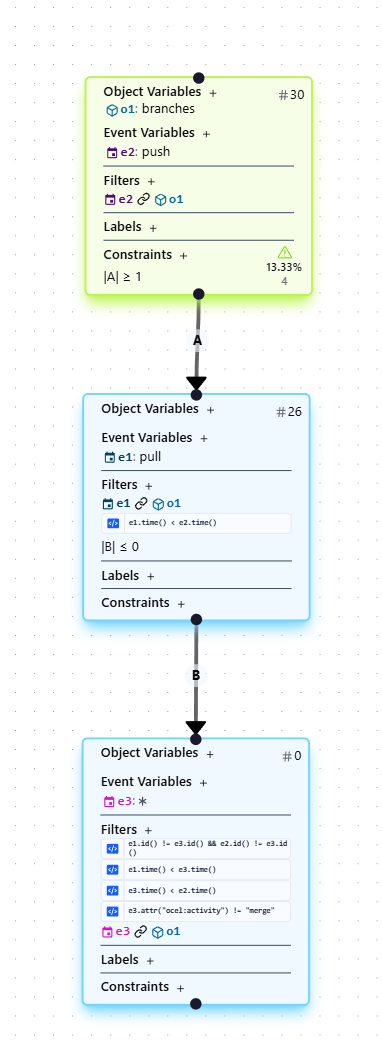
\includegraphics[width=0.8\textwidth,height=0.5\textheight,keepaspectratio]{figures/c1_query_screenshot.png}
      \caption{OCPQ query for C1 (three nested nodes) and result: 4 of 30 pushes violate C1
            (86.67\% compliance).}
      \label{fig:c1-query}
\end{figure}

\paragraph{Result and explanation.} The query flags 4 of the 30 pushes as violations (see
Figure~\ref{fig:c1-query}). A push is only counted as compliant if it has an \emph{immediately}
preceding pull on the same branch, with no event other than a merge in between; existence of some
\emph{earlier}, non-adjacent pull is not sufficient, since anything (including another push or
commit) sitting between that pull and the push disqualifies it as a witness. The four flagged
pushes either have no preceding pull on their branch at all, or every earlier pull is separated
from them by an intervening non-merge event.

% -------------------------------------------------------------------
\subsubsection*{C2: ``Do not alternate between branches: after committing to one branch $b$,
      you should not touch a different branch until having pushed to $b$.''}

\paragraph{Query.} Again a three-level nested query tree.

\begin{itemize}
      \item \textbf{Root node} -- all commits: variables $e_1 : \text{commit}$,
            $o_1 : \text{branches}$, $o_2 : \text{users}$;
            filters $\mathrm{E2O}(e_1, o_1)$, $\mathrm{E2O}(e_1, o_2)$.
      \item \textbf{Child node} -- candidate later pushes to the same branch by the same user:
            variable $e_2 : \text{push}$ (inherits $o_1$, $o_2$);
            filters $\mathrm{E2O}(e_2, o_1)$, $\mathrm{E2O}(e_2, o_2)$,
            \texttt{e1.time() < e2.time()}.
      \item \textbf{Grandchild node} -- events by the same user on a \emph{different} branch,
            strictly between $e_1$ and this candidate push:
            variable $e_3 : *$, $o_3 : \text{branches}$;
            filters $\mathrm{E2O}(e_3, o_2)$, $\mathrm{E2O}(e_3, o_3)$,
            \texttt{o3.id() != o1.id()},
            \texttt{e1.time() < e3.time()},
            \texttt{e3.time() < e2.time()}.
\end{itemize}

Constraints: on the \emph{child} (push) node we require $|\text{grandchild}| \le 0$, keeping only
pushes to $b$ that are not preceded by activity of the same user on a different branch. On the
\emph{root} (commit) node we require $|\text{child}| \ge 1$: a commit is compliant iff at least
one such clean push exists afterwards.

\begin{figure}[h]
      \centering
      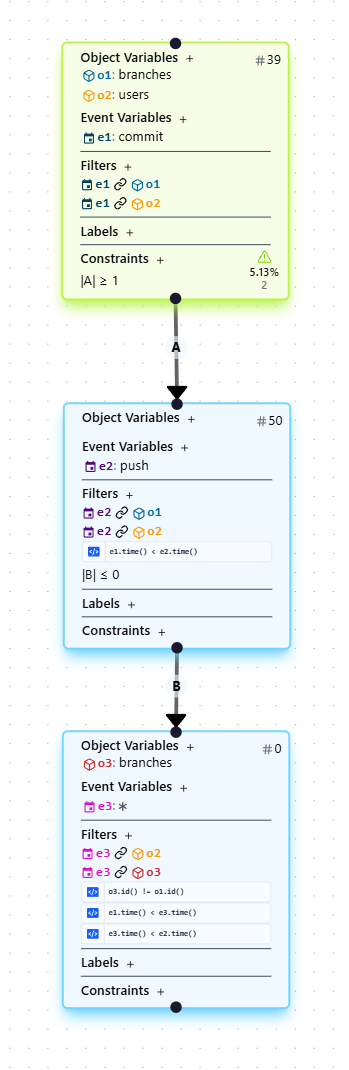
\includegraphics[width=0.8\textwidth,height=0.5\textheight,keepaspectratio]{figures/c2_query_screenshot.png}
      \caption{OCPQ query for C2 (three nested nodes) and result: 2 of 39 commits violate C2
            (94.87\% compliance).}
      \label{fig:c2-query}
\end{figure}

\paragraph{Result and explanation.} 2 of the 39 commits violate C2 (see
Figure~\ref{fig:c2-query}). A commit is compliant if the committing user eventually pushes to the
same branch again without first touching a different branch; committing again, or pulling, on
the \emph{same} branch $b$ in between does not count against the constraint, only activity tied
to a \emph{different} branch object does. Of the two violating commits, at least one case
corresponds to the user touching a different branch before ever pushing to $b$; the other case
may correspond to the user never pushing to $b$ again at all -- both are genuine violations of
C2, but for different underlying reasons.

% -------------------------------------------------------------------
\subsubsection*{C3: ``Avoid coordination problems: a coordination problem between two users
      $u_1 \neq u_2$ is a merge event that consumes two versions of the same file, where one version
      was committed by $u_1$ and the other by $u_2$.''}

\paragraph{Query.} Unlike C1 and C2, C3 is not an existential (``does a witness exist'')
condition but a direct pattern match, so a single flat query node suffices.

\begin{itemize}
      \item Object variables: $o_1, o_2 : \text{file versions}$, $o_3 : \text{files}$,
            $o_4, o_5 : \text{users}$.
      \item Event variables: $e_1 : \text{merge}$, $e_2, e_3 : \text{commit}$.
      \item Filters:
            $\mathrm{E2O}(e_1, o_1)$@consume, $\mathrm{E2O}(e_1, o_2)$@consume,
            $\mathrm{O2O}(o_1, o_3)$@is\_a, $\mathrm{O2O}(o_2, o_3)$@is\_a,
            $\mathrm{E2O}(e_2, o_1)$@produce, $\mathrm{E2O}(e_3, o_2)$@produce,
            $\mathrm{E2O}(e_2, o_4)$, $\mathrm{E2O}(e_3, o_5)$;
            CEL constraints \texttt{o1.id() < o2.id()} and \texttt{o4.id() != o5.id()}.
\end{itemize}

The condition \texttt{o1.id() < o2.id()} imposes a canonical ordering on the two conflicting
versions so that each real coordination problem is counted exactly once (without it, every
coordination problem would be found twice, as $(o_1,o_2)$ and $(o_2,o_1)$). The condition
\texttt{o4.id() != o5.id()} is the actual C3 condition: the two versions were committed by
different users.

\begin{figure}[h]
      \centering
      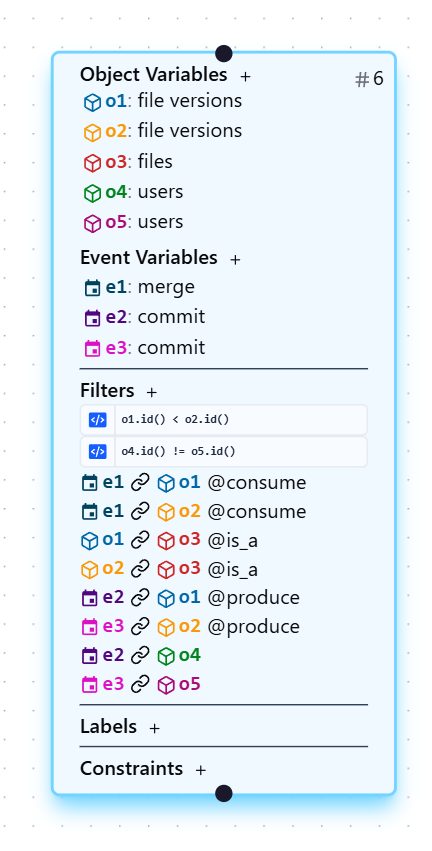
\includegraphics[width=0.8\textwidth,height=0.5\textheight,keepaspectratio]{figures/c3_query_screenshot.png}
      \caption{OCPQ query for C3 (single flat node) and result: 6 coordination problems found.}
      \label{fig:c3-query}
\end{figure}

\paragraph{Result and explanation.} The query returns 6 output bindings (see
Figure~\ref{fig:c3-query}), i.e. 6 coordination problems: pairs of file versions of the same
file, produced by two different users, that were both consumed by the same merge event. Each
binding directly witnesses one instance of the pattern described by C3, so no separate
compliance percentage is computed here -- the count itself is the answer. Note that this counts
\emph{version pairs}; if a single merge consumed more than two conflicting versions it would
contribute multiple pairs to this count rather than being counted once per merge.

% Q5b: Flattening-based conformance checking for Cameron
% ─────────────────────────────────────────────────────────────────────────────
% Results produced by q5b_conformance.py.
% ─────────────────────────────────────────────────────────────────────────────

\subsection{(b) Conformance checking for Cameron}
\label{sec:q5b}
\begin{figure}[H]
      \centering
      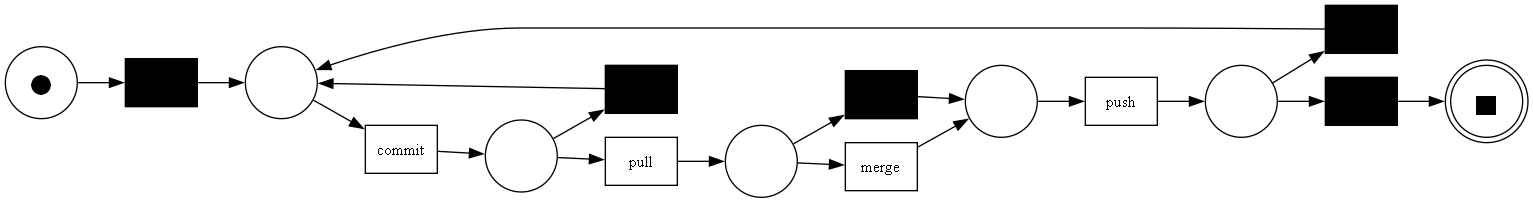
\includegraphics[width=0.6\textwidth,height=0.35\textheight,keepaspectratio]{figures/n1_subnet_model.png}
      \caption{Per-object-type subnet of \None{} (identical for \otBranches{} and
            \otUsers{}): $\etCommit^+ \to \etPull \to [\etMerge]? \to \etPush$,
            looped. Generated by \texttt{q5b\_conformance.py} (\texttt{build\_n1\_subnet}).}
      \label{fig:n1}
\end{figure}

Applying the given definition of \logLuone{} for $u=\userCameron$
(\texttt{q5b\_conformance.py}) yields 13 events, flattened below per object type.

\subsubsection*{Flattened traces}

\begin{table}[H]
      \centering\small
      \caption{Traces per branch (\otBranches{} flattening of \logLuone{}).}
      \label{tab:traces-branches}
      \begin{tabularx}{\textwidth}{@{}lX@{}}
            \toprule
            \textbf{Branch} & \textbf{Trace}                                                          \\
            \midrule
            b1              & commit $\to$ pull $\to$ push $\to$ commit $\to$ push $\to$ commit $\to$
            commit $\to$ commit $\to$ pull $\to$ push                                                 \\
            b3              & commit $\to$ pull $\to$ push                                            \\
            \bottomrule
      \end{tabularx}
\end{table}

\begin{table}[H]
      \centering\small
      \caption{Trace for \userCameron{} (\otUsers{} flattening of \logLuone{}).}
      \label{tab:traces-users}
      \begin{tabularx}{\textwidth}{@{}lX@{}}
            \toprule
            \textbf{User} & \textbf{Trace}                                                          \\
            \midrule
            Cameron       & commit $\to$ pull $\to$ push $\to$ commit $\to$ push $\to$ commit $\to$
            commit $\to$ commit $\to$ pull $\to$ push $\to$ commit $\to$ pull $\to$ push            \\
            \bottomrule
      \end{tabularx}
\end{table}

\subsubsection*{Token-based replay fitness}

Computed with \texttt{pm4py.conformance\_diagnostics\_token\_based\_replay}
against \cref{fig:n1}.

\begin{table}[H]
      \centering\small
      \caption{Token replay diagnostics — \otBranches{} subnet.}
      \label{tab:replay-branches}
      \begin{tabular}{@{}lcccccc@{}}
            \toprule
            \textbf{Trace (branch)} & \textbf{Fit?}     & \textbf{Fitness} &
            \textbf{Consumed}       & \textbf{Produced} & \textbf{Missing} & \textbf{Remaining}              \\
            \midrule
            b1                      & No                & 0.9474           & 19                 & 19 & 1 & 1 \\
            b3                      & Yes               & 1.0000           & 7                  & 7  & 0 & 0 \\
            \midrule
            \textbf{Average}        &                   & \textbf{0.9737}  &                    &    &   &   \\
            \bottomrule
      \end{tabular}
\end{table}

\begin{table}[H]
      \centering\small
      \caption{Token replay diagnostics — \otUsers{} subnet.}
      \label{tab:replay-users}
      \begin{tabular}{@{}lcccccc@{}}
            \toprule
            \textbf{Trace (user)} & \textbf{Fit?}     & \textbf{Fitness} &
            \textbf{Consumed}     & \textbf{Produced} & \textbf{Missing} & \textbf{Remaining}              \\
            \midrule
            Cameron               & No                & 0.9583           & 24                 & 24 & 1 & 1 \\
            \midrule
            \textbf{Average}      &                   & \textbf{0.9583}  &                    &    &   &   \\
            \bottomrule
      \end{tabular}
\end{table}

$\bar{f} = \frac{f_{\text{branches}} + f_{\text{users}}}{2}
      = \frac{0.9737 + 0.9583}{2} = 0.9660$.

\subsubsection*{Alignments}
\label{sec:q5b-alignments}

Computed with \texttt{pm4py.conformance\_diagnostics\_alignments}. A plain
activity is a synchronous move, \texttt{tau} a silent model move, and
\texttt{(log:X)} a log-only move (deviation).

\begin{itemize}\footnotesize\raggedright
      \item \texttt{b1} (fitness $0.9231$):
            \texttt{tau commit pull tau push tau commit tau (log:push) commit tau
                  commit tau commit pull tau push tau}
      \item \texttt{b3} (fitness $1.0000$):
            \texttt{tau commit pull tau push tau}
      \item Cameron / \otUsers{} (fitness $0.9375$):
            \texttt{tau commit pull tau push tau commit tau (log:push) commit tau
                  commit tau commit pull tau push tau commit pull tau push tau}
\end{itemize}

Average alignment fitness: $0.9615$ (\otBranches), $0.9375$ (\otUsers).
Both non-fit traces share the same single \texttt{(log:push)} deviation, which
is the source of the missing/remaining token in
\cref{tab:replay-branches,tab:replay-users} (used for C1 below).

\subsubsection*{Alignment-based precision (prefix automata)}

Reconstructed via the Align-ET Conformance algorithm (Adriansyah et al., 2015):
one node per log prefix, solid edges for activities the log continues with,
dashed red edges for activities \None{} would additionally allow but that never
occur (escaping edges, which reduce precision).

\begin{figure}[H]
      \centering
      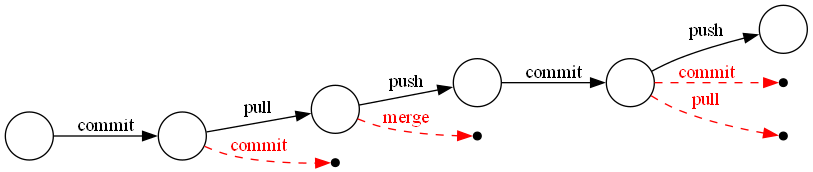
\includegraphics[width=0.85\textwidth,height=0.3\textheight,keepaspectratio]{figures/prefix_automaton_branches.png}
      \caption{Prefix automaton — \otBranches{} subnet.}
      \label{fig:prefix-branches}
\end{figure}

\begin{figure}[H]
      \centering
      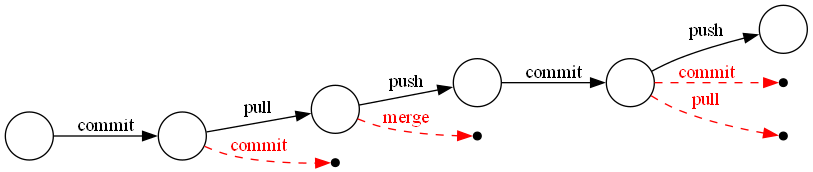
\includegraphics[width=0.85\textwidth,height=0.3\textheight,keepaspectratio]{figures/prefix_automaton_users.png}
      \caption{Prefix automaton — \otUsers{} subnet.}
      \label{fig:prefix-users}
\end{figure}

$\bar{p} = \frac{p_{\text{branches}} + p_{\text{users}}}{2}
      = \frac{0.5385 + 0.5000}{2} = 0.5192$.

\subsubsection*{Fitness and precision summary}

\begin{table}[H]
      \centering\small
      \caption{Aggregated conformance results for \logLuone{} vs.\ \None.}
      \label{tab:conformance-summary}
      \begin{tabular}{@{}lcc@{}}
            \toprule
            \textbf{Subnet}  & \textbf{Token-replay fitness} & \textbf{Alignment precision} \\
            \midrule
            \otBranches      & 0.9737                        & 0.5385                       \\
            \otUsers         & 0.9583                        & 0.5000                       \\
            \midrule
            \textbf{Average} & \textbf{0.9660}               & \textbf{0.5192}              \\
            \bottomrule
      \end{tabular}
\end{table}

\subsubsection*{Checking C1 and C2 for Cameron}

\paragraph{C1 (pull before push).}
Yes. \None{} encodes C1 directly ($\etPush$ is only enabled after a $\etPull$ of
the current round), so the single deviation found in both subnets \emph{is} a C1
violation: the alignment pinpoints it as the \texttt{b1} push at event
\texttt{e82}, occurring right after a commit with no intervening pull -- matching
the violation independently found in Q5a(a).

\paragraph{C2 (no branch-switching after commit).}
No. \None's \otBranches{} subnet checks each branch in isolation and the
\otUsers{} subnet discards branch identity, so neither can tell that an event
belongs to a \emph{different} branch than the one currently active -- exactly
what C2 requires. Indeed, \userCameron{} committed to \texttt{b3} (event
\texttt{e89}) while \texttt{b1} was still unpushed, a genuine C2 violation, yet
it causes no missing/remaining token in either subnet; detecting it needs a query
that keeps both object types in scope simultaneously, as in Q5a(a).

\end{document}
